\documentclass[journal]{IEEEtran}

\usepackage[T1]{fontenc}
\usepackage[utf8]{inputenc}
\usepackage{amsmath,amssymb,amsfonts}
\usepackage{graphicx}
\usepackage{booktabs}
\usepackage{array}
\usepackage{url}
\usepackage{xcolor}
\usepackage[hidelinks]{hyperref}
\usepackage{orcidlink}
\usepackage{balance}

\graphicspath{{../figures/}}

\renewcommand{\topfraction}{0.92}
\renewcommand{\bottomfraction}{0.75}
\renewcommand{\textfraction}{0.08}
\renewcommand{\floatpagefraction}{0.80}

% IEEEtran hard-codes an em-dash after the abstract and index-terms names; the CAOS
% content standard (ADR-0067) excludes em-dashes, so the separator is a full stop.
\makeatletter
\def\abstract{\normalfont
    \if@twocolumn
      \@IEEEabskeysecsize\bfseries\textit{\abstractname}.\ \relax
    \else
      \bgroup\par\addvspace{0.5\baselineskip}\centering\vspace{-1.78ex}\@IEEEabskeysecsize\textbf{\abstractname}\par\addvspace{0.5\baselineskip}\egroup\quotation\@IEEEabskeysecsize
    \fi\@IEEEgobbleleadPARNLSP}
\def\IEEEkeywords{\normalfont
    \if@twocolumn
      \@IEEEabskeysecsize\bfseries\textit{\IEEEkeywordsname}.\ \relax
    \else
      \bgroup\par\addvspace{0.5\baselineskip}\centering\@IEEEabskeysecsize\textbf{\IEEEkeywordsname}\par\addvspace{0.5\baselineskip}\egroup\quotation\@IEEEabskeysecsize
    \fi\@IEEEgobbleleadPARNLSP}
\makeatother

% Page-1 header block (conventions/manuscript-header-standard.md). The four document
% macros are set by the publishing tool when the version DOI is reserved.
\newcommand{\doctype}{Technical report}
\newcommand{\docversion}{v1.1}
\newcommand{\docdate}{18 September 2026}
\newcommand{\versiondoi}{10.5281/zenodo.22823062}
\newcommand{\conceptdoi}{10.5281/zenodo.21519007}
\newcommand{\docrepo}{github.com/fsantibanezleal/CAOS\_ProspectMap}
\newcommand{\headerblock}{%
\begin{center}
\fbox{\parbox{0.94\textwidth}{\small\raggedright
\textbf{\doctype} \quad$\cdot$\quad \docversion, \docdate \quad$\cdot$\quad Licence CC BY 4.0\\[2pt]
CAOS open-research programme \quad$\cdot$\quad CAOS\_ProspectMap, mineral prospectivity mapping\\[2pt]
Version DOI \href{https://doi.org/\versiondoi}{\texttt{\versiondoi}} \quad$\cdot$\quad
concept DOI (always latest) \href{https://doi.org/\conceptdoi}{\texttt{\conceptdoi}}\\[2pt]
Not peer reviewed. Source code, data and computational records: \href{https://\docrepo}{\texttt{\docrepo}}
}}
\end{center}}

\begin{document}

\title{ProspectMap: The Two Ways a Mineral\\ Prospectivity Map Lies, Quantified on the\\ Real US Mississippi-Valley-Type Belt}

\author{Felipe~Santiba\~nez-Leal~\orcidlink{0000-0002-0150-3246}%
\thanks{F. Santiba\~nez-Leal is with the CAOS open-research programme, Santiago, Chile
(e-mail: fsantibanez@gmail.com; ORCID 0000-0002-0150-3246).}%
\thanks{Interactive tool and reproducible pipeline (MIT) at
\url{https://github.com/fsantibanezleal/CAOS_ProspectMap}; the tool is available at
\url{https://prospectmap.fasl-work.com}.}}

% The leading {} lets IEEEtran's \MakeUppercase reach \doctype, so the whole head is set in capitals.
\markboth{{}\doctype\ \docversion, 2026}%
{Santiba\~nez-Leal: The two ways a mineral prospectivity map lies}

\IEEEaftertitletext{\vspace{-0.6\baselineskip}\headerblock\vspace{0.2\baselineskip}}

\maketitle

\begin{abstract}
A mineral prospectivity map stacks geophysical, geochemical and structural evidence over a study area and outputs,
per cell, the probability that a deposit is there. Such maps are typically presented with an area-under-curve
(AUC) and a posterior, and both numbers can be inflated in two specific, well-understood ways.
ProspectMap is an interactive tool that computes such a map by Weights of Evidence, a Bayesian log-odds update,
and makes those two inflations \emph{first-class}, measuring them rather than hiding them. This report quantifies
both on the real US Midcontinent Mississippi-Valley-type zinc-lead belt (the open Critical Minerals Mapping
Initiative dataset of Lawley \emph{et al.}, 2022) and on ten synthetic terranes. The first inflation is
\emph{evaluation}: reporting AUC under random cross-validation, which lets spatially adjacent cells leak between
train and test, overstates prospective skill; on the real belt the Weights-of-Evidence AUC, scored over all map
cells, falls from $0.72$ under random cross-validation to $0.64$ under spatial block cross-validation (an
inflation of $0.09$, the largest of any case), and a learned classifier, scored on a labelled sample of deposit
cells and distance-buffered non-deposit cells, drops from $0.98$ to $0.95$. The spatial estimate is the one to
report; the two models' spatial-CV AUCs come from different cell sets and are not a like-for-like comparison. The
second inflation is \emph{modelling}: Weights of Evidence assumes the evidence layers are conditionally independent given
a deposit, and it reports large contrasts that look decisive, but on the real belt those contrasts are
statistically \emph{insignificant}, every layer's studentized contrast is below the $95\%$ threshold, so the
confident-looking weights do not survive their own error bars. The tool displays both corrected diagnostics, the
spatial-CV AUC and the studentized significance, beside the inflated values; every number and figure can be
regenerated from the released artifacts.
\end{abstract}

\begin{IEEEkeywords}
Mineral prospectivity, Weights of Evidence, conditional independence, spatial cross-validation, AUC inflation,
Mississippi-Valley-type, critical minerals, model evaluation, reproducibility.
\end{IEEEkeywords}

\section{Introduction}

\IEEEPARstart{W}{here} is the next ore deposit most likely to be? Mineral prospectivity mapping answers it by
overlaying evidence layers, a magnetic high here, a geochemical anomaly there, proximity to a favourable
structure, over a study-area grid and computing, per cell, a posterior probability of a deposit. The classical
method is Weights of Evidence~\cite{bonham94,bonham89}: each binary evidence pattern gets a positive weight
$W^+$ where it is present and $W^-$ where it is absent, their difference is the contrast $C=W^+-W^-$, and the
posterior log-odds of a deposit in a cell is the prior log-odds plus the sum of the present-or-absent weights.
The output is a map, and the map is usually reported with two numbers: a high area-under-curve showing it separates
known deposits from barren ground, and confident-looking weights. Both are, in a well-documented way, prone to
inflation.

ProspectMap is a tool built to expose the inflation. It computes the Weights-of-Evidence
posterior live, and it makes first-class the two ways the numbers lie. The first is that an AUC reported under
\emph{random} cross-validation is optimistic, because a prospectivity grid is spatially autocorrelated and a
random split leaves near-neighbour cells in both train and test, so the model is partly tested on what it has
seen; \emph{spatial} cross-validation, holding out contiguous blocks, gives a realistic estimate~\cite{roberts}. The
second is that Weights of Evidence assumes the evidence layers are conditionally independent given a deposit, and
when they are not the posterior is overconfident~\cite{agterberg}; and even when the contrasts look large, they
may not be statistically significant. This report quantifies both, on the real US Mississippi-Valley-type
zinc-lead belt from the open Critical Minerals Mapping Initiative dataset~\cite{lawley} and on ten synthetic
terranes, and reports a modern learned classifier~\cite{rodriguez} under the same random-versus-spatial
contrast. The contribution is the measurement and the display of the two
inflations, not a new prospectivity algorithm.

% Defined before Section II so that the full-width float lands at the top of the next page.
\begin{figure*}[!t]
\centering
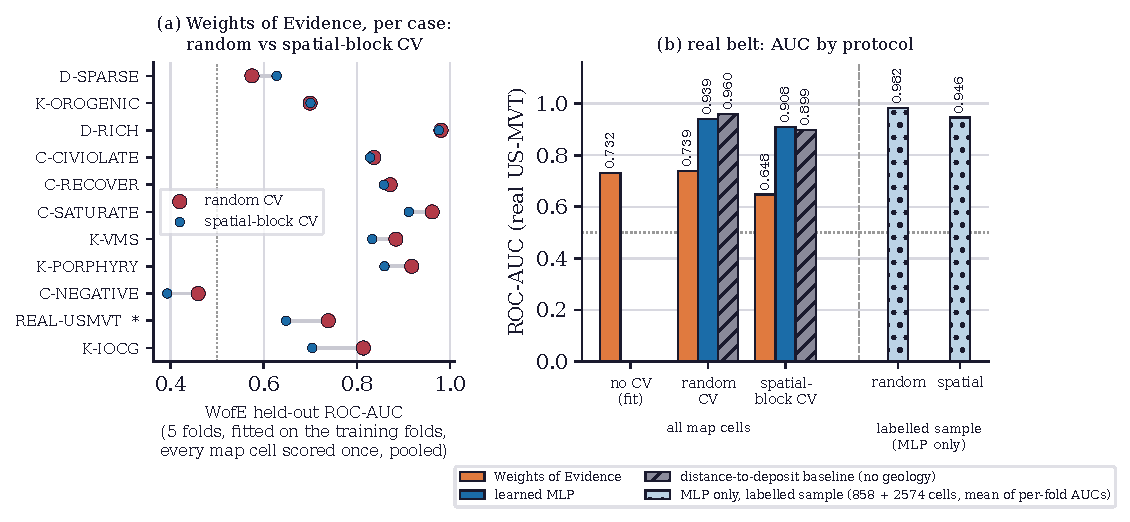
\includegraphics[width=0.84\textwidth]{fig-inflation.pdf}
\caption{The evaluation inflation. \textbf{(a)} Weights-of-Evidence AUC under random versus spatial
cross-validation, per case (five folds; spatial folds are $20\times20$-cell blocks; every map cell scored): random
cross-validation (red) is at least as high as spatial (blue) in every case except D-RICH, where spatial exceeds
random by $0.001$, because adjacent cells leak; the gap is largest on the real US-MVT belt (marked $*$), where the
AUC falls from $0.72$ to $0.64$. Spatial cross-validation gives the realistic estimate. \textbf{(b)} The real belt,
AUC by protocol: Weights of Evidence scored over all map cells without cross-validation ($0.732$, weights fitted
on all deposits), under random ($0.723$) and under spatial ($0.637$) cross-validation; the learned classifier
scored on its labelled sample (the 858 deposit cells and 2574 sampled non-deposit cells more than two cells from
any deposit) under random ($0.982$) and spatial ($0.946$) cross-validation. The two models are scored on
different cell sets, so their AUCs are not directly comparable.}
\label{fig:inflation}
\end{figure*}

\section{The First Lie: Cross-Validation Inflation}\label{sec:cv}

The first inflation is a matter of how the map is scored, and it is quantified in Fig.~\ref{fig:inflation}a. For
every case, the Weights-of-Evidence posterior is evaluated two ways: random five-fold cross-validation, which
splits the grid cells at random, and spatial five-fold cross-validation, which holds out contiguous
$20\times20$-cell blocks so that the test set is geographically separate from the training set; in both, the
weights are refitted on the training folds' deposits and every map cell receives a held-out score. Random
cross-validation is at least as optimistic in every case but D-RICH, where the spatial AUC is higher by $0.001$,
because a prospectivity grid is strongly spatially autocorrelated and a random split leaves a test
cell's near neighbours in the training set, so the model is scored partly on cells like ones it has seen. The gap
is real and, on the \emph{real} US Mississippi-Valley-type belt, it is the largest of any case: the
Weights-of-Evidence AUC falls from $0.723$ under random cross-validation to $0.637$ under spatial, an inflation of
$0.087$. A learned classifier, a small multilayer perceptron on the six continuous evidence layers (Weights of
Evidence uses their binarized patterns), cross-validated with the same block size and fold count but scored on a
labelled sample of the 858 deposit cells and 2574 sampled non-deposit cells more than two cells from any deposit,
falls from $0.982$ to $0.946$. The spatial estimate is the relevant one; the random one overstates how well the
map would find a deposit in unseen ground. Fig.~\ref{fig:inflation}b
sets these values beside the Weights-of-Evidence AUC without cross-validation ($0.732$, weights fitted and scored
on the whole map). The spatial-CV AUCs of the learned classifier ($0.946$) and of Weights of Evidence ($0.637$)
are computed on different cell sets and averaged differently (the mean of per-fold AUCs for the classifier,
pooled held-out scores for Weights of Evidence), so their difference is not a like-for-like comparison of the two
methods.

\section{The Second Lie: Overconfident Weights}\label{sec:woe}

\begin{figure*}[!t]
\centering
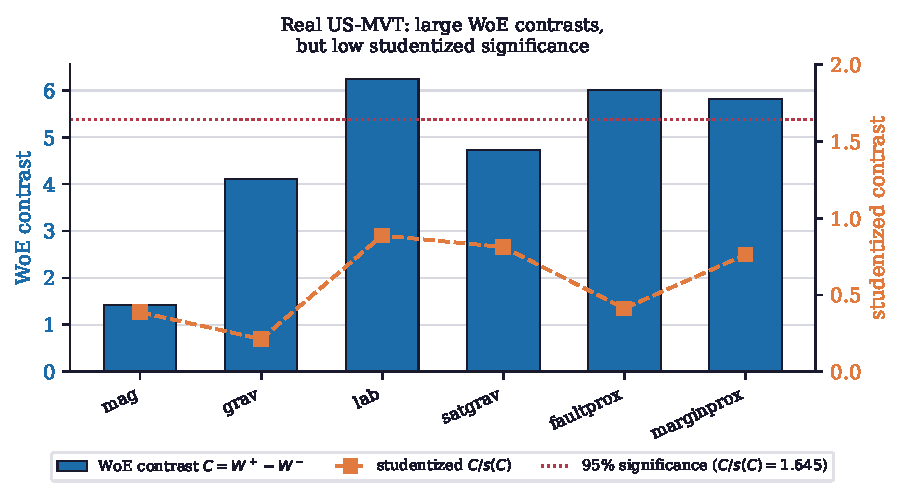
\includegraphics[width=0.66\textwidth]{fig-woe.pdf}
\caption{The modelling inflation. Weights-of-Evidence contrasts $C=W^+-W^-$ (bars) and their studentized
significance $C/s(C)$ (line) for the six evidence layers of the real US-MVT belt. The raw contrasts are large
(up to $6$), which looks decisive, but every layer's studentized contrast is below the $95\%$ significance
threshold of $1.645$: on real, sparse deposit data the weights carry large standard errors and are not
statistically significant, so the confident-looking map rests on evidence that does not survive its own error
bars.}
\label{fig:woe}
\end{figure*}

The second inflation is in the weights themselves (Fig.~\ref{fig:woe}). Weights of Evidence assumes the evidence
layers are conditionally independent given a deposit; when correlated layers are stacked, their weights
double-count the same signal and the posterior becomes overconfident, which is why a conditional-independence
test~\cite{agterberg} belongs in any Weights-of-Evidence workflow, and ProspectMap runs one. But there is a
simpler and equally important check that is often skipped: whether a contrast is statistically significant at all. On the real US-MVT
belt the six evidence layers have large raw contrasts, up to about $6$, which a practitioner reading only the
contrast would take as strong evidence. Their studentized contrasts $C/s(C)$, however, are all between $0.2$ and
$0.9$, well below the $1.645$ threshold for $95\%$ significance: with sparse deposits and noisy layers the
standard error of each weight is large, and none of the contrasts clears its own error bar. The map
built from them may still be useful for ranking, but presenting its weights as decisive evidence is the second
way the map lies, and showing the studentized contrast beside the raw one is the correction.

\section{Discussion and Scope}\label{sec:discuss}

The two inflations are independent and both matter. A map can have significant weights and still report an
inflated AUC because it was scored with random cross-validation; or it can have a spatially cross-validated AUC
and still oversell weights that are not significant. ProspectMap's contribution is to compute the
Weights-of-Evidence map and then put the deflating diagnostics next to it, the spatial-CV AUC beside the random
one, the studentized contrast beside the raw one, and a conditional-independence test, so a user sees the
corrected diagnostics beside the inflated ones, and a learned classifier is reported under the same
random-versus-spatial contrast ($0.982$ against $0.946$ on its labelled sample). The ten terrane cases are synthetic,
used to exercise the diagnostics under known ground truth; the one real case is the open Critical Minerals
Mapping Initiative US-MVT dataset~\cite{lawley}, a real belt, on which spatial cross-validation
removes the largest AUC inflation of any case and no evidence layer's contrast is significant. The tool is a
decision-support and teaching instrument, not an exploration recommendation for any specific ground; it says where
the evidence points and, more importantly, how much to trust it. The interface shows the same diagnostics on
every map.

\section{Conclusion}

A mineral prospectivity map lies in two well-understood ways: it reports an AUC inflated by random
cross-validation, and it presents Weights-of-Evidence contrasts that look decisive but may violate conditional
independence or fail their own significance test. ProspectMap measures both. On the real US Mississippi-Valley-type
belt the Weights-of-Evidence AUC falls from $0.72$ to $0.64$ when scored by spatial cross-validation (the largest
inflation of any case), a learned classifier scored on a labelled sample falls from $0.98$ to $0.95$ under the
same switch from random to spatial cross-validation, and every evidence layer's contrast is statistically
insignificant despite looking large. The contribution
is a reproducible tool that displays the corrected diagnostics, spatial-CV AUC and studentized significance, next
to the inflated ones.

\appendices
\section{Reproduction}\label{app:repro}

{\raggedright\setlength{\parindent}{1em}
The repository artifacts under \path{data/derived/} carry each case's Weights-of-Evidence layers (contrasts and
studentized contrasts), posterior summary, pairwise conditional-independence tests, and both random- and
spatial-cross-validation AUC (\path{case-results.json}), together with the learned classifier's random- and
spatial-CV AUCs on the real belt (\path{pm-learned-real.json}, whose field \path{spatial_cv.wofe_roc_auc} holds the
Weights-of-Evidence AUC without cross-validation) and the real US-MVT trace (\texttt{REAL-USMVT}, with the Lawley
\emph{et al.} provenance). The figure scripts under \path{manuscripts/prospectivity/figures/} read those
artifacts; the pipeline is seeded, so re-running reproduces Fig.~\ref{fig:inflation} and Fig.~\ref{fig:woe}.\par}

\balance

\begin{thebibliography}{00}

\bibitem{bonham89} G.~F. Bonham-Carter, F.~P. Agterberg, and D.~F. Wright, ``Weights of evidence modelling: A new
approach to mapping mineral potential,'' in \emph{Statistical Applications in the Earth Sciences}, Geological
Survey of Canada Paper 89-9, 1989, pp.~171--183.

\bibitem{bonham94} G.~F. Bonham-Carter, \emph{Geographic Information Systems for Geoscientists: Modelling with
GIS}. Oxford: Pergamon, 1994.

\bibitem{agterberg} F.~P. Agterberg and Q.~Cheng, ``Conditional independence test for weights-of-evidence
modeling,'' \emph{Natural Resources Research}, vol.~11, no.~4, pp.~249--255, 2002.
doi:10.1023/A:1021193827501.

\bibitem{lawley} C.~J.~M. Lawley \emph{et al.}, ``Data-driven prospectivity modelling of sediment-hosted Zn-Pb
mineral systems and their critical raw materials,'' \emph{Ore Geology Reviews}, vol.~141, art.~104635, 2022.
doi:10.1016/j.oregeorev.2021.104635.

\bibitem{roberts} D.~R. Roberts \emph{et al.}, ``Cross-validation strategies for data with temporal, spatial,
hierarchical, or phylogenetic structure,'' \emph{Ecography}, vol.~40, no.~8, pp.~913--929, 2017.
doi:10.1111/ecog.02881.

\bibitem{rodriguez} V.~Rodriguez-Galiano, M.~Sanchez-Castillo, M.~Chica-Olmo, and M.~Chica-Rivas, ``Machine
learning predictive models for mineral prospectivity: An evaluation of neural networks, random forest, regression
trees and support vector machines,'' \emph{Ore Geology Reviews}, vol.~71, pp.~804--818, 2015.
doi:10.1016/j.oregeorev.2015.01.001.

\end{thebibliography}

\end{document}
